%Modified from a template provided by Jennifer Pan, August 2011

\documentclass[10pt,letter]{article}
	% basic article document class
	% use percent signs to make comments to yourself -- they will not show up.
\usepackage{pdfsync}
\usepackage{amsmath}
\usepackage{amssymb}
\usepackage{amsthm}
\usepackage{ mathrsfs }
	% packages that allow mathematical formatting

\usepackage{graphicx}
	% package that allows you to include graphics
\graphicspath{ {./images/} }

\usepackage{setspace}
	% package that allows you to change spacing

\onehalfspacing
	% text become 1.5 spaced

\usepackage{fullpage}
% package that specifies normal margins

\usepackage[parfill]{parskip}

\usepackage{cancel}

\newtheorem*{thm}{Theorem}
\newtheorem{nthm}{Theorem}

\begin{document}
	% line of code telling latex that your document is beginning

\title{Problem Set 6: CS103}

\author{Katherine Cheng, Richard Davis, Marty Keil}

% \date{Friday April 10, 2015}
	% Note: when you omit this command, the current date is automatically included
 
\maketitle
	% tells latex to follow your header (e.g., title, author) commands.

\section*{Problem 1: The Myhill-Nerode Theorem}
\paragraph{i}
\begin{thm} L is a regular language, where $\Sigma = \{a,b\}$ and $L=\{w \in \Sigma^* |\ |w| \text{ is even}\}$\end{thm}
\begin{proof}

Let $\Sigma = \{a,b\}$ and let $L=\{w \in \Sigma^* |\ |w| \text{ is even}\}$. We can design DFA for this language:

\begin{figure}[h]
    \centering
    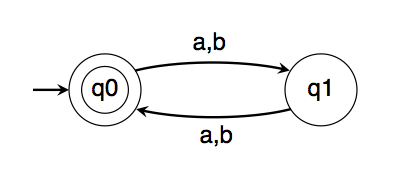
\includegraphics[width=0.4\linewidth]{hw6_1i.png}
    \caption{DFA for the language $L=\{w \in \Sigma^* |\ |w| \text{ is even}\}$ where $\Sigma = \{a,b\}$}
    \label{fig:q1i}
\end{figure}

As defined in lecture, we know that a language $L$ is a regular language if there exists a DFA $D$ such that $\mathscr{L}(D) =L$. Thus, L must be a regular language.
\end{proof}

\paragraph{ii}
\begin{thm} There is an infinite set $S \subseteq \Sigma^*$ where there are infinitely many pairs of distinct strings $x, y \in S$ such that $x\ \cancel{\equiv}_L\ y$ \end{thm}

\begin{proof}
Let $S= \{a^n\ |\ n \in \mathbb{N}\}$. This set is infinite because it contains one string for each natural number. Since $a^n$ is the string $a$ concatenated to itself $n$ times, we know the length of $a^n$ is $n$. Now, consider any pair of strings $a^n, a^{n+1} \in S$. The lengths of these strings are $n$ and $n+1$ respectively. By the definition of even and odd numbers, if $n$ is even, $n+1$ must be odd. If $n$ is odd, $n+1$ must be even. In either case, one string in the pair must be even-length and in the language $L$, and the other odd-length and not in the language $L$, meaning that $a^n\ \cancel{\equiv}_L\ a^{n+1}$. There are infinite such pairs, thus, S has infinitely many pairs of distinct strings.
\end{proof}

\paragraph{iii}
\begin{thm} There is no infinite set $S \subseteq \Sigma^*$ where all pairs of distinct strings $x,y\in S$ satisfy $x\ \cancel{\equiv}_L\ y$ \end{thm}

\begin{proof}
By contradiction. Suppose there is an infinite set $S \subseteq \Sigma^*$ where all pairs of distinct strings $x,y \in S$ satisfy $x\ \cancel{\equiv}_L\ y$. We know that every string must be of even or odd length. If we take any three distinct strings from the infinite set S, by the pigeonhole principle, we know that two of these strings are of odd length, or two of these strings are of even length. Thus, we have found a pair of distinct strings where $x \equiv_L y$. We have reached a contradiction, so our original assumption must be false. Thus, there is no infinite set $S \subseteq \Sigma^*$ where all pairs of distinct strings $x,y\in S$ satisfy $x\ \cancel{\equiv}_L\ y$
\end{proof}

\section*{Problem 2: Balanced Parentheses}
\paragraph{i}
\thm The Language L = ( $w \in ?*$ | w is a string of balanced parentheses ) is not regular. 

\proof Let $S = (,)*.$ This set is infinite because it contains one parentheses for each natural number. There is some infinite subset S which is the $(^n$. One can add w (a closed parentheses equal to the number of either string x open parentheses or string y open parentheses) and one is in the language and another is not in the language.  Consequently X is distinguishable from y. Therefore, by the Myhill-Nerode theorem, L is not regular. 

\paragraph{ii}
Online

\paragraph{iii}
S ? (A | ?
A ? )S | (B
B ? )A | (C
C ? )B | (D
D ? )C

\section*{Problem 3: Subsets of Regular Languages}
Let $\Sigma = \{a, b\}$ and let $L = \{ w \in \Sigma^* \ | \ w \text{ has the same number of a's and b's} \}$. 
\paragraph{i} 

\proof Sigma star is all possible combination you can make. $a^n$ is the subset of these strings, which is infinite. For any pair you wind a w, in which  X and y are distinguishable. Therefore, by the Myhill-Nerode theorem, L is not regular. 

\paragraph{ii}
(ab)*. You can write a DFA for it and it is infinite. 

\paragraph{iii}
$A^nB^n$ is irregular which means that every pair is pairwise distinguishable. So any subset of it must also be pairwise distinguishable. So since this subset is infinite and pairwise distinguishable, it is a irregular language. However, since this contradicts the the assumption that both are regular. 

\section*{Problem 4: State Lower Bounds}
\paragraph{i}
\begin{thm}Any DFA for L, where L is a language over $\Sigma$ and there's a finite set S such that any two distinct strings $x,y\in S$ are distinguishable relative to L, must have at least $|S|$ states. \end{thm}

\begin{proof} Let the number of strings in set S, $|S| = k$. Since all pairs of distinct strings x and y are pairwise distinguishable relative to L, by the definition of distinguishability discussed in lecture, any DFA for L must end in different states when run on inputs x and y. If every input string leads the DFA for L to end in a different state from every other string, each input string must lead the DFA to a unique state. Thus, if there are k strings in set S, there are at least k states in the DFA for L. Substituting $|S|$ back in for k, this means that any DFA for L must have at least $|S|$ states.
\end{proof}

\paragraph{ii}
\begin{thm} The following DFA is the smallest possible DFA for L, where L is a language over $\Sigma = \{a,b\}$ and $L=\{w \in \Sigma^*\ |\ |w| \equiv_4 2\}$.\end{thm}

\begin{figure}[h]
    \centering
    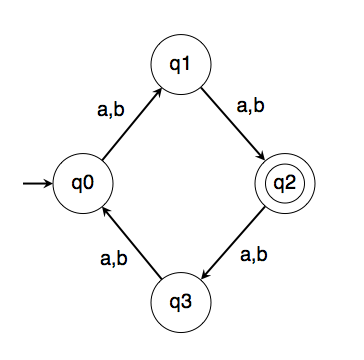
\includegraphics[width=0.4\linewidth]{hw6_4ii.png}
    \caption{DFA for the language $L=\{w \in \Sigma^*\ |\ |w| \equiv_4 2\}$ where $\Sigma = \{a,b\}$}
    \label{fig:q4ii}
\end{figure}

\begin{proof} Assume L is a language over $\Sigma = \{a,b\}$ and $L=\{w \in \Sigma^*\ |\ |w| \equiv_4 2\}$. We will show that the DFA modeled here is the smallest possible DFA for L, the measure of ``smallest" being the number of states in the DFA (which, in this DFA, is 4 states). 

Take the finite set, $S = \{a^1, a^2, a^3, a^4\}$. We can take any pair of strings $a^n, a^m \in S$ and add a string w to each, where $w = a^{6-n}$. Adding w to these strings will lead exactly one string, $a^n + w = a^n+a^{6-n} = a^6$, to be in L ($a^6 \equiv_4 2$), and the other not to be in L. Thus, as defined in lecture, the strings $a^n, a^m \in S$ are distinguishable relative to L. Since this is true of any pair of strings in S, the strings in this finite set are all pairwise distinguishable relative to L.

By our proof in Part i of this problem, since we have shown there is a finite set S such that all strings in the set are pairwise distinguishable relative to L, there must be at least $|S|$ states in the DFA for L. The cardinality of our set S is 4, so there must be at least 4 states in the DFA for L. Therefore, our DFA depicted above must be the smallest possible DFA for L. 
\end{proof}

\section*{Problem 5: Closure Properties Revisited}
\paragraph{i}
Proof. if and only if statement. Therefore if its irregular and regular this cannot be the case. Any tie the complement or the language itself is regular, the other must be regular. So anytime the language is irregular, then the complement must also be regular. 

\paragraph{ii}
Disproof, can have single accepts state f l2 is the complement of L1. Now the union is accepts any string, so is just one accepting state. 

\paragraph{iii}
Disproof by existence. For ab, aabb, all are individual strings, when infinite, becomes an irregular language. 

\section*{Problem 6: Designing CFGs}
\paragraph{i}
S ? ? | XaSaX
X ? ? | bX | cX | aX

\paragraph{ii}
I spent way too long on this. But it is wrong...
S ? ? | XaSbY | bSa
X ? ? | aXb | Xa
Y ? ? | aYb | Yb

S ? baX | ZabY | ?
X ? Xa | XbaY | bbX | abW | ?
Z ? Zab | Za | ?
Y ? bY | ?
W ? ab

\paragraph{iii}


\paragraph{vi}
Start symbol: S
S ? aSXXX | bXXX | SXXXX
X ? a | b

\paragraph{v}
S ? ydS | Sdy | dSy | ySd | ZySyZ | XdSdX | ?
Z ? d
X ? y
\end{document}
%%% Local Variables:
%%% mode: latex
%%% TeX-master: t
%%% End:
